
\section{Additive Faithfulness}

For general regression, additive approximation may result in a
relevant variable being incorrectly marked as irrelevant. Such
mistakes are inherent to the approximation and may persist even with
infinite samples.  In this section we give
examples of this phenomenon, and then show how the convexity
assumption
changes the behavior of the additive approximation.  We begin
with a lemma that implies uniqueness of the additive regression function.


\begin{figure*}[htp]
\vskip-10pt
	\centering
	\subfigure[egg carton]{
		\centering
		{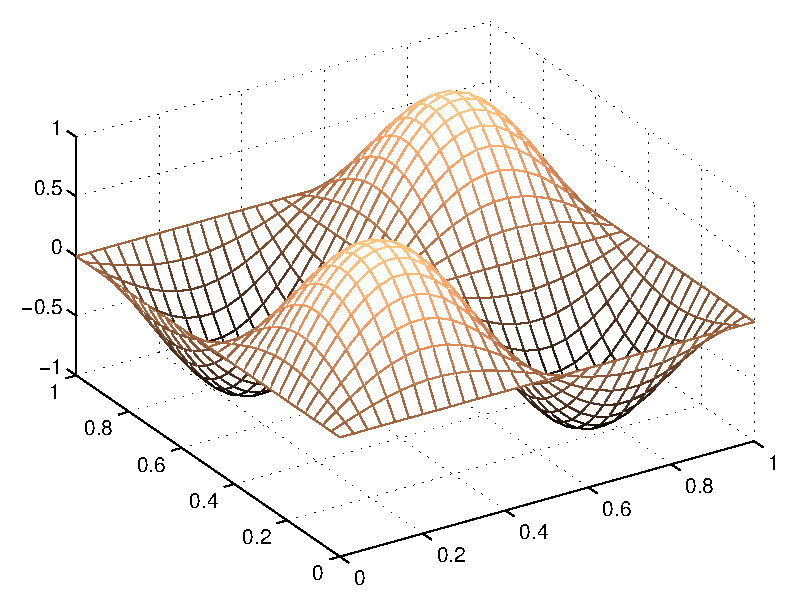
\includegraphics[width=0.4\textwidth]{../figs/sine_wave_funct3}}
	}
	\subfigure[tilting slope]{
		\centering
		{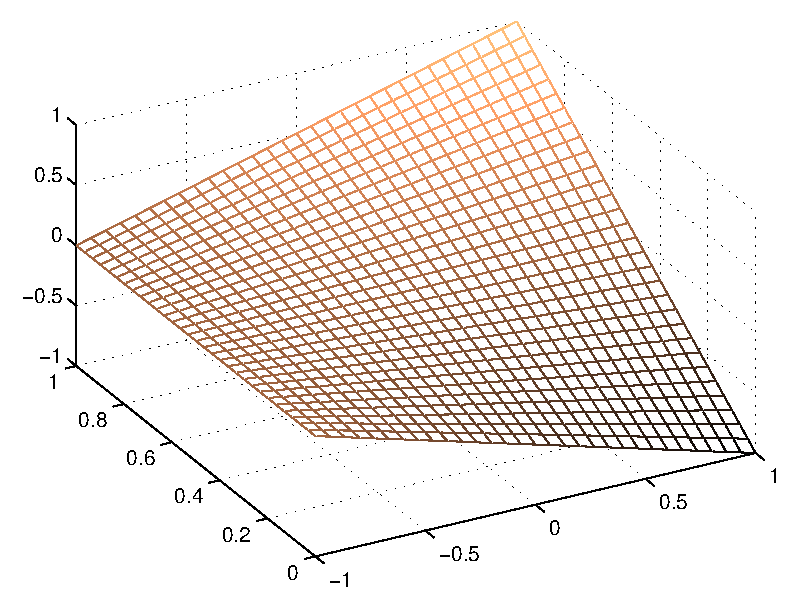
\includegraphics[width=0.4\textwidth]{../figs/tilting_slope_funct3}}
	}
\caption{Two additively unfaithful functions. Relevant variables are
  zeroed out under an additive approximation because every ``slice''
  of the function integrates to zero.}
\vskip-10pt
\end{figure*}


\begin{lemma}
\label{lem:general_int_reduction}
Let $F$ be a product distribution on $\mathbf{C}=[0,1]^s$ with density function $p$ which is positive on $\mathbf{C}$. Let
$X=(X_1,...,X_s) \sim F$. Let $f: \mathbf{C} \rightarrow \R$ be an
integrable function.
Let 
\begin{equation}
\begin{split}
f_k^*, \mu^* \coloneqq \argmin_{f_1,\ldots, f_s, \mu} \Bigl\{ \E \bigl( f(X) & -
 \sum_{k=1}^s f_k(X_k) -\mu \bigr)^2 \\
       & \,:\, \E f_k(X_k) = 0\Bigr\}.
\end{split}
\end{equation}
Then $\mu^* = \E f(X)$ and $f^*_k(x_k) = \E[ f(X) \given x_k] - \E f(X)$ and this solution is unique.
\end{lemma}

Lemma~\ref{lem:general_int_reduction} follows from the stationarity
conditions of the optimal solution. If $F$ is the uniform distribution,
then $f^*_k(x_k) = \int f(x_k, \mathbf{x}_{-k})
d\mathbf{x}_{-k}$.

\begin{example} We give two examples of additive unfaithfulness under
  the uniform distribution. First, consider the following function:
\[
\trm{(egg carton)} \quad f(x_1, x_2) = \sin( 2\pi x_1) \sin( 2 \pi x_2)
\]
defined for $(x_1, x_2) \in [0,1]^2$.  Then
$\int_{x_2} f(x_1, x_2) d x_2 = 0$ and
$\int_{x_1} f(x_1, x_2) d x_1 = 0$ for each $x_1$ and $x_2$. An additive approximation
would set $f_1 = 0$ and $f_2 = 0$.  Next, consider the function
\[
\trm{(tilting slope)} \quad f(x_1, x_2) = x_1 x_2
\]
defined for $x_1 \in [-1,1],\; x_2 \in [0,1]$.  In this case
$\int_{x_1} f(x_1, x_2) d x_1 = 0$ for each $x_2$; therefore, we expect $f_2 = 0$ under the additive approximation. This function, for every fixed $x_2$, is a zero-intercept linear function of $x_1$ with slope $x_2$.
\end{example}

In order to exploit additive models, it is important to understand when the
additive approximation accurately captures all of the relevant variables.
We call this property \emph{additive faithfulness}.

\begin{definition}
  Let $\mathbf{C}=[0,1]^s$, and $f:\mathbf{C}\rightarrow \R$. We say
  that $f$ \emph{depends on} coordinate $k$ if there exist $x'_k \neq
  x_k$ such that $f(x'_k, \mathbf{x}_{-k})$ and $f(x_k,
  \mathbf{x}_{-k})$ are different functions of $\mathbf{x}_{-k}$.

Let $F$ be a probability distribution on $\mathbf{C}$ and
assume without loss of generality that $\E f(X) = 0$. Let 
\begin{equation}
\begin{split}
f_k^*, \mu^* \coloneqq \argmin_{f_1,\ldots, f_s, \mu} \Bigl\{ 
             \E ( f(X) &- \sum_{k=1}^s f_k(X_k) -\mu )^2 \\
         &\,:\, \E f_k(X_k) = 0 \Bigr\}.
\end{split}
\end{equation}
We say that $f$ is \emph{additively faithful} under $F$ in case $f^*_k = 0$ iff $f$ does not depend on coordinate $k$. 
\end{definition}
% We can define the support $\trm{supp}(f) \coloneqq \{ k \,:\,
% \trm{$k$ is relevant to $f$}\}$. Let $f^* = \sum_{k=1}^s$, then $f$
% is additively faith if $\trm{supp}(f) = \trm{supp}(f^*)$.

Remarkably, under product distributions, a convex multivariate function can always be faithfully approximated by an additive function. 

\begin{theorem}
\label{thm:convex_faithful}
Let $F$ be a product distribution supported on $C=[0,1]^s$ with positive density $p$. If $f$ is convex and twice differentiable, then $f$ is additively faithful under $F$.
\end{theorem}

We give the full proof in Section~\ref{sec:faithful_proof} of the
Appendix, but pause here to provide some intuition. From
Lemma~\ref{lem:general_int_reduction}, we know that the
additive approximation zeroes out $k$ when, fixing $x_k$, every
``slice'' of $f$ integrates to zero. We prove
Theorem~\ref{thm:convex_faithful} by showing that ``slices'' of convex
functions that integrate to zero cannot be ``glued'' together while
still maintaining convexity.

Theorem~\ref{thm:convex_faithful} plays an important role in our
sparsistency analysis, where we show that the additive
approximation is variable selection consistent (or ``sparsistent''), even when the true function is not
additive.

\begin{remark}
  We assume twice differentiability in
  Theorem~\ref{thm:convex_faithful} to simplify the proof. We believe
  this smoothness condition is not necessary because every non-smooth
  convex function can be approximated arbitrarily well by a smooth
  one.  Without restrictions on the distribution, a convex
  function may not be additively faithful. Intuitively, an arbitrarily shaped
  density $p$
  may ``undo'' the convexity of $f$ so that the product
  $p(\mathbf{x}) \, f(\mathbf{x})$ resembles an egg carton or a
  tilting slope.  With appropriate conditions on the density $p$,
  however, it is possible to relax the independence assumption.  We leave this to
  future work.
\end{remark}
